%\documentclass[10pt,a4paper]{report}
%\usepackage[utf8]{inputenc}
%\usepackage[german]{babel}
%\usepackage{amsmath}
%\usepackage{amsfonts}
%\usepackage{amssymb}
%\usepackage{graphicx}

%\begin{document}
	\chapter{Grundlagen der Quantenmechanik}
		\section{Klassische Mechanik}
			\subsection{Kinematik}

				\begin{itemize}
					\item System. z.b Planet, geladenes Teilchen, elektromagn. Feld
					\item Observable $\hat{=}$ Messgrössen,	z.B.:
					
					\begin{description}
						 \item \(\vec{x}, \vec{v},\vec{p},E=\dfrac{1}{2}m\left|\vec{v}\right|^{2} \)
						 \item \( \vec{B}, \vec{E}, E=\int_{-\infty}^{\infty} \D^3x (\vec{E}^2+\vec{B}^2)\)
						 \item \( \vec{P}=\int_{-\infty}^{\infty}  \D^3 x (\vec{E} \times \vec{B})\)
					\end{description}                   
                           
					\item Zustand: vollständige Information zu einem Zeitpunkt t des Systems, z.B.: 
					\begin{description}
						 \item \((\vec{x_i},\vec{p_i}) \), i=1,...,N  \space (N Teilchen, Massen m)
						 \item \( (\vec{E},\vec{B})\)
					 \end{description}        
					 \item $\{ Observable\} \rightarrow \{reelle Zahl\}$
					 \item alle Funktionen von Obervablen sind Observable             
				\end{itemize}

				\subsection{Dynamik(Zeitentwicklung, Vorhersagen)}
					\begin{itemize}
						\item spezifische Wechselwirkungen $\rightsquigarrow$ Kräfte, Potentiale, Lagrange, Hamilton,\\
						Bewegungsgleichungen $\vec{F}=m \cdot \vec{a}$, $\vec{F_G}=-G\dfrac{m_1m_2}{r^2}\dfrac{\vec{r}}{r}$
						\item Vorhersagen(deterministisch): gegeben $ (\vec{x},\vec{p})$ für t=0 kann $(\vec{x}(t), \vec{p}(t))$ berechnet werden
						\item vollständig (!)
					\end{itemize}


				\subsection{Weltbild der klassischen Physik vor ca. 1900}
					\begin{itemize}
						\item insgesamt ausreichend für experimentelle Befunde
						\item Materie (Newton etc.) $\neq$ Strahlung (Elektromagnetismus)
						\item Verknüpfung über Lorentzkraft
					\end{itemize}

				\section{Physik als Würfel}
					\begin{center}
						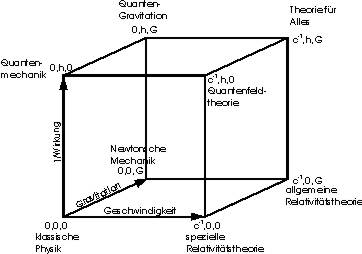
\includegraphics[scale=2]{wurfel.jpg}
					\end{center}

				\section{Unvollständigkeit der KM und Elektrodynamik}
					\underline{Beispiele:}
					\begin{enumerate} 
						\item Stabilität der Materie: $T_stabil >> $ 1 Tag
						\begin{itemize}
							\item $E(\vec{x},\vec{p})=\dfrac{\vec{p}^2}{2m}-\dfrac{e^2}{r}$
							\item $E(\vec{x}, 0) =- \dfrac {e^2}{r}$ unbeschränkt nach unten
							\item instabil bei Störungen, Strahlung (!)
						\end{itemize}
					      	$\Rightarrow T_{stabil} << 10^{-30} s$
						\item kontinuierliches Spektrum vorhergesagt, diskretes beobachtet
						\item Lichtquanten
						\begin{itemize}
							\item Planck 1900: Hohlraumstrahlung, E-M-Welle $E=n\cdot(h\cdot \nu)$,\\ $h=6,7*10^{-34} Js$
							\item Einstein 1903: Photoeffekt: Korpuskulartheorie
							\item Einstein-de-Broglie:
							\boxed{E=h\nu=\hbar\omega \mbox{, } p=\hbar\vec{k}}, $\|\vec{k}\|=\dfrac{2\pi}{\lambda}$, $p=\dfrac{h}{\lambda}$
							\item zum Photoeffekt: \\ Energie der Strahlung $E_{Licht}=\int_{-\infty}^{\infty} \D^3x (\vec{E}^2+\vec{B}^2)$erwartet klassisch $E_{Licht} \propto E_{Elektron}$, Überraschung: $E_{Elektron} \propto \nu_{Licht}$
							\item 1905: Strahlung als Teilchen, Photon erklärt
							\item 1924: Compton-Effekt
						\end{itemize}
						\item Materiewellen
						\begin{itemize}
							\item de Broglie: $ \lambda = \frac{h}{|\vec{p}|} $
							\item 1923 für materielle Teilchen
							\item 1927 Elektronenbeugungsversuch (Nobelpreis 1937)
							\item \underline{Beispiel:} Staubkorn \\
									$ d = 1 \mu m, \ m = 10^{-15}kg, \ v=1 \frac{mm}{s} $ \\
									$ \Rightarrow \lambda = \frac{h}{m \cdot v} = 10^{-15}m $ 
						\end{itemize}
					\end{enumerate}
					
				\section{Welle-Teilchen-Dualität}
					Doppelspaltversuch in verschiedenen Ausführungen:
					\begin{itemize}
						\item Klassisch: 
						\begin{itemize}
							\item Die E-Felder addieren sich: $ \vec{E} = \vec{E}_1 + \vec{E}_2 $
							\item Es kommt zu einem Interferenzmuster
							\item Nur ein Spalt führt zu keinem Interferenzmuster
						\end{itemize}
						\item Mit $ e^- $ als Quelle:
						\begin{itemize}
							\item Einfachspalt führt zu keinem Interferenzmuster
							\item Klassische Erwartung für Teilchen: $ P = P_1 + P_2$, Addition der Wahrscheinlichkeiten
							\item Experiment: $ P \neq P_1 + P_2  $
						\end{itemize}
						\item Verdünnte Strahl $ \rightarrow $ einzelne Lichtquanten, räumlich getrennt
						\begin{itemize}
							\item Klassische Erwartung für Welle: Interferenz mit $ I \rightarrow 0 $ (Falsch)
							\item Resultat: Photon interferiert mit sich selbst
						\end{itemize}
						\item Ortsvermessung durch Blockieren eines Spalts oder Detektor am Spalt.
						\begin{itemize}
							\item Ortsmessung $ \rightarrow $ keine Interferenz (Impulsmessung)
							\item Interferenzmessung $ \rightarrow $ keine Ortsmessung am Spalt
						\end{itemize}
						$ \Longrightarrow $ Welle-Teilchen-Dualität, Auflösung in der QM mit Wellenfunktion $ \psi(\vec{r}, t) \in \mathbb{C} $ und Wahrscheinlichkeit $ | \psi |^2 $
						\item Zusammenfassung: 
						\begin{itemize}
							\item Zustand - Wahrscheinlichkeitsamplitude\\ $ P = |A|^2 $ $ P_1=|A_1|^2  P_2=|A_2|^2 $\\ $P = |A_1 + A_2|^2 = |A_1|^2 + |A_2|^2 + A_1\bar{A_2} + \bar{A_1}A_2$
							\item Nicht alle Variablen haben exakte Werte in einem Zustand: Zufall! Keine klassische statistische Verteilung.
							\item klassisch: $ \vec{E} $ beliebig, QM: $ E = n  h  \nu $
							\item Blockieren eines Spalts entspricht Ortsmessung
							\item Messung eines Interferenzmusters entspricht der Bestimmung von Impuls/Wellenlängen
						\end{itemize}
					\end{itemize}
					
				\section{Postulate der QM}
					\subsection{Bedeutung von $\Psi$}
						\begin{itemize}
							\item $ \Psi(\vec{r},t): \mathbb{R}^3 \times \mathbb{R} \rightarrow \mathbb{C}$
							\item Wahrscheinlichkeitsamplitude $ \D P(\vec{r},t) = C*|\Psi|^2 \D^3 r $. Wahrscheinlichkeit, dass Teilchen zum Zeitpunkt $ t $ in $ \D^3r $ um Punkt $ \vec{r} $ zu finden ist.
							\item \underline{Bem:} 
							\begin{itemize}
								\item C=Normierung
								\item $  \int \D P(\vec{r},t) = 1$, Irgendwo befindet sich das Teilchen \\
									$ \Longrightarrow $ $ \int |\Psi|^2 \D^3r = \frac{1}{C}$
								\item Schrödingergleichung: $ \frac{\D C}{\D t} = 0 $
							\end{itemize}
						\end{itemize}
						
						\subsection{Messung}
							\begin{itemize}
								\item Ergebnisse nach Wahrscheinlichkeitsverteilung
								\item Kollaps der Wellenfunktion(Punktaufschlag)
								\item Messwerte: Eigenwerte von Operatoren auf dem Raum der W.fkt. 
							\end{itemize}
						
						\subsection{Schrödingergleichung}
							\begin{itemize}
								\item $i \hbar \frac{\partial \Psi(\vec{r}, t)}{\partial t} = \H(\vec{r},t)\Psi(\vec{r}, t)$
								\item ohne Hamiltonoperator $i \hbar \frac{\partial \Psi(\vec{r}, t)}{\partial t} = \frac{- \hbar ^2}{2m} \Delta \Psi(\vec{r}, t) + V(\vec{r}, t) \Psi(\vec{r}, t)$
							\end{itemize}
								\subsection{Quantisierungsregeln}
							\begin{itemize}
							\item KM: x Koordinate $\looparrowright$ X Operator
							\item $\{~, \}~~\looparrowright$ [~,~]
							\item Hamiltonsche Form der KM $\looparrowright$ Schrödinger Gleichung
							\item \underline{Bemerkung:}
							\begin{itemize}
							\item Was ist real?
							\begin{align*}
							\vec{r}(t):\text{ 3 Zahlen } \looparrowright \Psi\left(\vec{r}, t\right):~~ \infty \text{ viele Zahlen}
							\end{align*}
							\item $\gamma$: erzeugt und vernichtet $\nLeftrightarrow$ Elektronen, Teilchen: bleiben erhalten
							\end{itemize}
							\end{itemize}
							\section{Freie Teilchen, Wellenpakete}
							\begin{itemize}
							\item potentielle Energie $V(\vec{r},t)=0~~\rightarrow$ kräftefrei
							\item Schrödinger-Gleichung:
							\begin{align*}
							i\hbar \frac{\partial}{\partial t}\Psi(\vec{r},t)=\frac{\hbar^2}{2m}\Delta\Psi(\vec{r},t)
							\end{align*}
							\item Lösungsansatz: ebene Welle
							\begin{align*}
							\Psi(\vec{r},t)&=A\cdot e^{i(\vec{k}\vec{r}-\omega t)}\\
							\frac{\partial}{\partial t}\Psi(\vec{r},t)&=-i\omega A e^{i(\vec{k}\vec{r}-\omega t)}=-i\omega\Psi\\
							\Delta\Psi(\vec{r},t)&=-Ae^{i(\vec{k}\vec{r}-\omega t)}\cdot k^2=-\Psi\cdot k^2\\
							\Rightarrow \hbar\omega\Psi(\vec{r},t)&=\frac{\hbar^2k^2}{2m}\Psi(\vec{r},t)\\
							\Rrightarrow \boxed{\omega=\frac{\hbar k^2}{2m}}
							\end{align*}
							$\Leftrightarrow$ Einstein-de Broglie-Bedingung:
							\begin{align*}
							E=\frac{p^2}{2m} \text{~~mit~} \vec{p}=\hbar\vec{k}
							\end{align*}
							\item $\omega(k)$ \textbf{Dispersionsrelation}
							\item ebene Welle nur Lösung, wenn Dispersionsrelation erfüllt ist
							\item Umkehrung:
							\begin{enumerate}[start=0]
							\item Einstein-de Broglie: $E=\hbar\omega$, $\vec{p}=\hbar\vec{k}$							
							\item klassisch: Energie des Teilchens: $E=\frac{p^2}{2m}$
							$\\\Rightarrow~~E=\frac{\hbar^2k^2}{2m}=\hbar\omega$
							\item ebene Wellen sollen Lösungen sein: Materiewelle $\Psi=Ae^{i(\vec{k}\vec{r}-\omega t)}$
							\item lineare PDE soll gelten:
							\begin{itemize}
							\item Wellengleichung: $\Box\Psi=0$ ?
							\item wegen $\omega \sim k^2~\leadsto~~\partial_t\Psi\sim\Delta\Psi~~\looparrowright$ z.B. Schrödinger-Gleichung
							\end{itemize} 
                            \end{enumerate}						
                            \item \underline{Bemerkung:}
                            \begin{itemize}
                   			\item $|\Psi(\vec{r},t)|^2=|A|^2$ konstante Wahrscheinlichkeit:
                   					\begin{align*}
               				 		\int |\Psi|^2dr^3~\rightarrow~\infty ~~\lightning   
									\end{align*}        
							\item unphysikalisch (wie in Optik!), nicht integrabel
							\item Lösung: Wellenpakete: Linearkombination ebener Wellen
									\begin{align*}
									\Psi(\vec{r}.t)=\frac{1}{(2\pi)^{2/3}} \int g(\vec{k})e^{i(\vec{k}\vec{r}-\omega(\vec{k})t)}d^3k
									\end{align*}
							\item jede quadratintegrable Wellenfunktion kann so geschrieben werden (Bedingung an $g(\vec{k})$)
							\item im eindimensionalen:
									\begin{align*}
									\Psi(\vec{r},t)=\frac{1}{\sqrt{2\pi}}\int\limits_{-\infty}^{\infty}g(k)e^{i(kx-\omega(k)t)}d^3k
									\end{align*}                
							\item Anfangswerte:
									\begin{align*}
									\Psi(x, 0)&=\frac{1}{\sqrt{2\pi}}\int\limits_{-\infty}^{\infty}e^{ikx}dk\\
g(k)&=\frac{1}{\sqrt{2\pi}}\int\limits_{-\infty}^{\infty}\Psi(x,0)e^{-ikx}dx
									\end{align*}
							\end{itemize}                            						 
					\item Form des Wellenpakets
					%Bild
					\item Spezialfall: $k_0, k_0-\frac{\Delta k}{2}, k_0+\frac{\Delta k}{2}$
							\begin{align*}
							\Psi(x)&=\frac{g(k_0)}{\sqrt{2\pi}}\left(e^{ik_0x}+\frac{1}{2}e^{i(k_0-\frac{\Delta k}{2})x}+\frac{1}{2}e^{i(k_0+\frac{\Delta k}{2})x}\right)\\
&=\frac{g(k_0)}{\sqrt{2\pi}}e^{ik_0x}\left(1+\cos\left(\frac{\Delta k}{2}x\right)\right)
							\end{align*}
					$\checkmark$ Paket, aber periodisch
					\item ''Unschärfe'': $\Psi(x)=0$ für $x=\pm\frac{\Delta x}{2}$ für Phasenunterschied $\pm\pi\\\leadsto\boxed{\Delta x\cdot\Delta k=4\pi}$
					\item später(allgemein):
							\begin{align*}
							\Delta x\cdot\Delta p&\geq\frac{\hbar}{2}~~~~~\text{(Heisenberg)}\\
							\text{statt:}~~~~\Delta x\cdot\Delta p&=4\pi\hbar~~(p=\hbar k)
							\end{align*}
					\item kohärente Welle:
							\begin{align*}
							\Delta x\cdot\Delta p=\frac{\pi}{2}
							\end{align*}
					\item Zeitliche Entwicklung (freies Wellenpaket):
							\begin{itemize}
							\item Phasengeschwindigkeit $e^{i(kx-\omega t)}$: $v_{\phi}(k)=									\frac{\omega}{k}$
							\item dispersives Medium: $v_{\phi}(k)=\frac{c}{n(k)}$ (vgl. Optik)
							\item Teilchenwelle: $v_{\phi}=\frac{\hbar k}{2m}$ wegen $\omega=\frac{\hbar k^2}{2m}$
							\item Gruppengeschwindigkeit: physikalisch! 

							(Signal, Energieausbreitung,...)
									\begin{itemize}
									\item Beispiel: 3 Wellen
											\begin{align*}
											\Psi(x,t)&=\frac{g(k_0)}{\sqrt{2\pi}}\left(e^{i(k_0x-\omega t)}+\frac{1}{2}e^{i((k_0-\frac{\Delta k}{2})x-(\omega_0-\frac{\Delta\omega}{2})t)}+\frac{1}{2}e^{i((...)x+(...)t)}\right)\\
											&=\frac{g(k_0)}{\sqrt{2\pi}}e^{i\underbrace{(k_0x-\omega_0t)}_{\text{Phase}}}\left[\underbrace{1+\cos\left(\frac{\Delta k}{2}x-\frac{\Delta\omega}{2}t\right)}_{\text{Gruppe}}\right]
											\end{align*}
									\item Maximum:
											\begin{align*}
											\boxed{x_m(t)=\frac{\Delta\omega}{\Delta k}t}
											\end{align*}
									%Bilder
									\end{itemize}
							\item allgemein: Gruppengeschwindigkeit ist Geschwindigkeit des \mbox{Maximums} des Wellenpakets
									\begin{align*}
									\boxed{v_G(k_0)=\left(\frac{\D\omega}{\D k}\right)_{k=k_0}}
									\end{align*}
							\item Teilchenwelle:
									\begin{align*}
									\boxed{v_G(k_0)=\frac{\hbar k_0}{m}=2v_{\phi}(k_0)}
									\end{align*}
							\end{itemize}
				\end{itemize}
							                
% \end{document}
